\section{Recorded-Trajectory Case Study}
\label{sec:recorded-results}

\subsection{Fixed-grid target-contract comparison}

On the one recorded fixed-grid waveform, scheduled P has position RMSE \RecordedBaselineRMSE, integer observed lag 20 ms, and sub-sample lag \RecordedPSubsampleLag. PV \FutureOOne{} at the vendor limits reduces RMSE to \RecordedPVRMSE, a \RecordedPVReductionPercent{} reduction on the same waveform. Its integer lag is \RecordedPVLag{} and its sub-sample lag is \RecordedPVSubsampleLag. The local trace in \cref{fig:recorded-case} shows a region selected by a deterministic rolling error-difference rule: PV follows the changing reference more closely than P without implying that every local interval improves.\claimtag{C9}

\begin{figure*}[t]
 \centering
 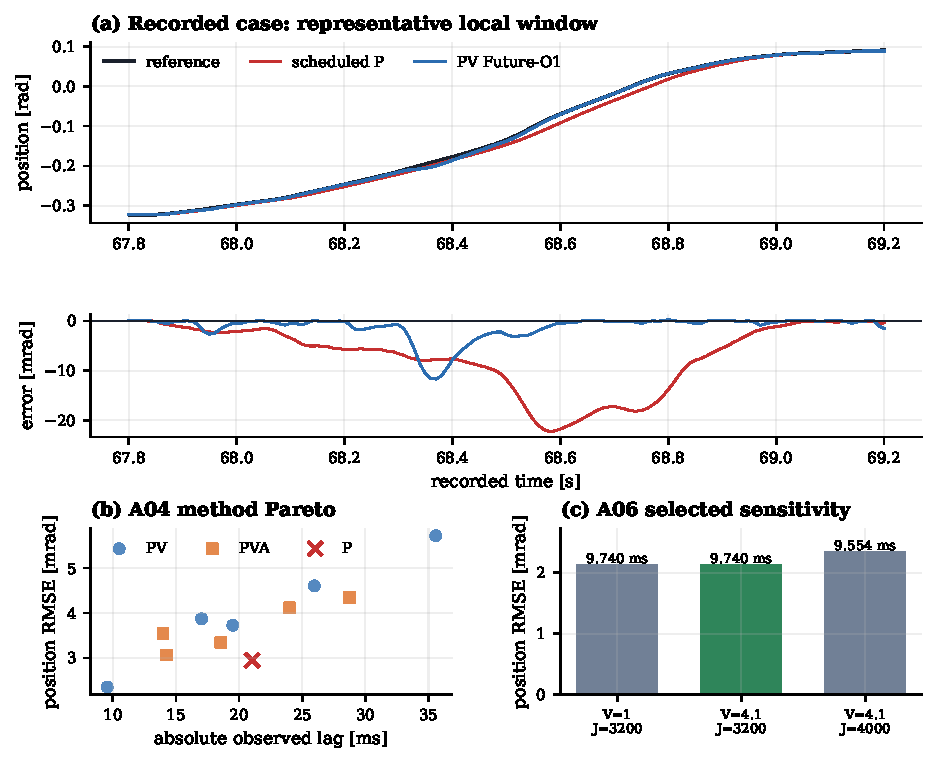
\includegraphics[width=\textwidth]{figures/generated/fig6_recorded_case.pdf}
 \caption{Recorded fixed-grid case study. (a) Reference, scheduled P, and PV \FutureOOne{} with position errors over a representative local window. (b) A04 RMSE--sub-sample-lag comparison for five PV and five PVA stencils, with P shown as a cross. (c) A06 sensitivity for the two performance-equivalent $J=3200$ settings and the $J=4000$ vendor reference. Lags are waveform-alignment diagnostics.}
 \label{fig:recorded-case}
\end{figure*}

PVA \FutureOOne{} does not improve this case. Its RMSE is \RecordedPVALRMSE, approximately \RecordedPVAIncreasePercent{} above scheduled P, while its integer lag is \RecordedPVALag{} and sub-sample lag is \RecordedPVASubsampleLag. This does not conflict with arbitrary-target-state OTG or with the value of acceleration targets in dynamic motion. It says that the particular causal acceleration construction and recorded waveform provide no net benefit under the current limits. Together with the constant-speed equivalence in A05, it prevents the acceleration field from being credited merely because it adds another component.\claimtag{C8}

One offline-host deadline miss occurred in the selected PV run, corresponding to one of \RecordedCycleCount{} evaluated cycles. Core kinematic constraints, solver completion, and target projection guardrails pass. Deadline is not used as the primary scientific gate, and this isolated diagnostic is not evidence of hardware real-time schedulability. A real-time claim would require a specified processor, operating system, scheduling policy, complete controller stack, and worst-case timing protocol.

\subsection{Vmax attribution}

A03 intervenes on the runtime velocity limit, changing it from $4.1$ to $10\ \mathrm{rad\,s^{-1}}$ for the same recorded inputs and PVA methods. For Future-O1, the log-ratio interaction of the PVA/P RMSE relationship is \VmaxInteraction, and acceleration projection counts remain unchanged. Across the tested stencils, relaxing runtime $V_{\max}$ does not remove the PVA deficit. The tested velocity condition becomes nonbinding while acceleration-related projection persists. We therefore reject runtime $V_{\max}$ as the explanation for the observed PVA degradation in this input and limit range. We do not claim that velocity limits are irrelevant in other tasks.\claimtag{C11}

\subsection{Best-tested VAJ setting}

A06 performs the second-stage engineering search after PV \FutureOOne{} has been selected. The deployment recommendation preserves the vendor velocity limit and uses $V/A/J=4.1/8.2/3200$. It achieves RMSE \RecordedBestRMSE, an improvement of \RecordedBestReductionPercent{} over scheduled P, with 10 ms integer lag, \RecordedBestSubsampleLag{} sub-sample lag, and zero target projection. The performance-equivalent $V=1$ setting has six projected targets, which is why it is not the deployment recommendation.\claimtag{C10}

The selected acceleration $A=8.2$ lies on the tested grid boundary, so the result is boundary-censored. It is the \emph{best tested} configuration, not a global optimum. Relative to the $J=4000$ vendor reference, $J=3200$ lowers RMSE by about \RecordedBestVsVendorReductionPercent{} while increasing sub-sample observed lag by approximately \RecordedBestLagTradeoff. The two co-primary metrics therefore retain a small trade-off that an integer-lag-only report would hide.

% Generated; do not edit.
\begin{table*}[t]
\centering
\caption{Recorded fixed-grid case study. Lags are observed waveform lags, not wall-clock latency. The deadline column is an offline-host guardrail.}
\label{tab:recorded}
\small
\begin{tabular}{@{}llllrrrrl@{}}
\toprule
Contract & Observer & $V/A/J$ & Role & RMSE [rad] & lag [ms] & sub-sample [ms] & projection & deadline \\
\midrule
P & none & $4.1/8.2/4000$ & baseline & 0.002951 & 20 & 21.029 & 0 & pass \\
PV & Future-O1 & $4.1/8.2/4000$ & method selection & 0.002352 & 10 & 9.554 & 0 & 1 miss \\
PVA & Future-O1 & $4.1/8.2/4000$ & negative result & 0.003536 & 10 & 13.976 & 0 & pass \\
PV & Future-O1 & $4.1/8.2/3200$ & best tested & 0.002129 & 10 & 9.740 & 0 & diagnostic \\
\bottomrule
\end{tabular}
\end{table*}

% Generated; do not edit.
\begin{table*}[t]
\centering
\caption{Robustness and negative controls. The recorded replay is diagnostic and is not an independent holdout.}
\label{tab:robustness}
\small
\begin{tabularx}{\textwidth}{@{}p{0.16\textwidth}p{0.17\textwidth}p{0.22\textwidth}X X@{}}
\toprule
Evidence & Evaluation unit & Result & Supports & Does not support \\
\midrule
E17 work envelope & 11 conditions, 1,320 pairs & all improve; weakest median 79.03\% & robustness in declared envelope & robot generalization \\
E17 stress diagnostics & 6 conditions, 720 pairs & noise 0.25 median 45.13\%, min. -10.63\% & visible envelope boundary & universal noise robustness \\
Synthetic trajectories & 20 trajectories & 20/20 pass; worst 98.67\% & tested nonconstant references & physical-task coverage \\
Recorded irregular replay & one waveform & local poly 0.003308 vs. P 0.002951 rad & explicit negative result & irregular-sampling remedy \\
\bottomrule
\end{tabularx}
\end{table*}


\Cref{tab:recorded} reports the recorded metrics and guardrails together. The
case study supports the mechanism at deployment-relevant scale without becoming
a generalization experiment. It contains one axis, one waveform, and no physical
plant. The causal comparison is A04's same-waveform target-contract intervention.
The additional A06 gain is an engineering selection layered on top; it must not
be attributed solely to the matched velocity target.
